\documentclass{article}

\usepackage{graphicx}
\usepackage{tikz}
\usepackage{tikzsymbols}
\usetikzlibrary{calc,patterns,shapes.geometric}
\pagestyle{empty}
\usepackage[margin=0pt]{geometry}
\geometry{papersize={14in,12in}}

\def\centerarc[#1](#2)(#3:#4:#5){\draw[#1] ($(#2)+({#5*cos(#3)},{#5*sin(#3)})$) arc (#3:#4:#5);}

\begin{document}
	\begin{figure}
		\centering
		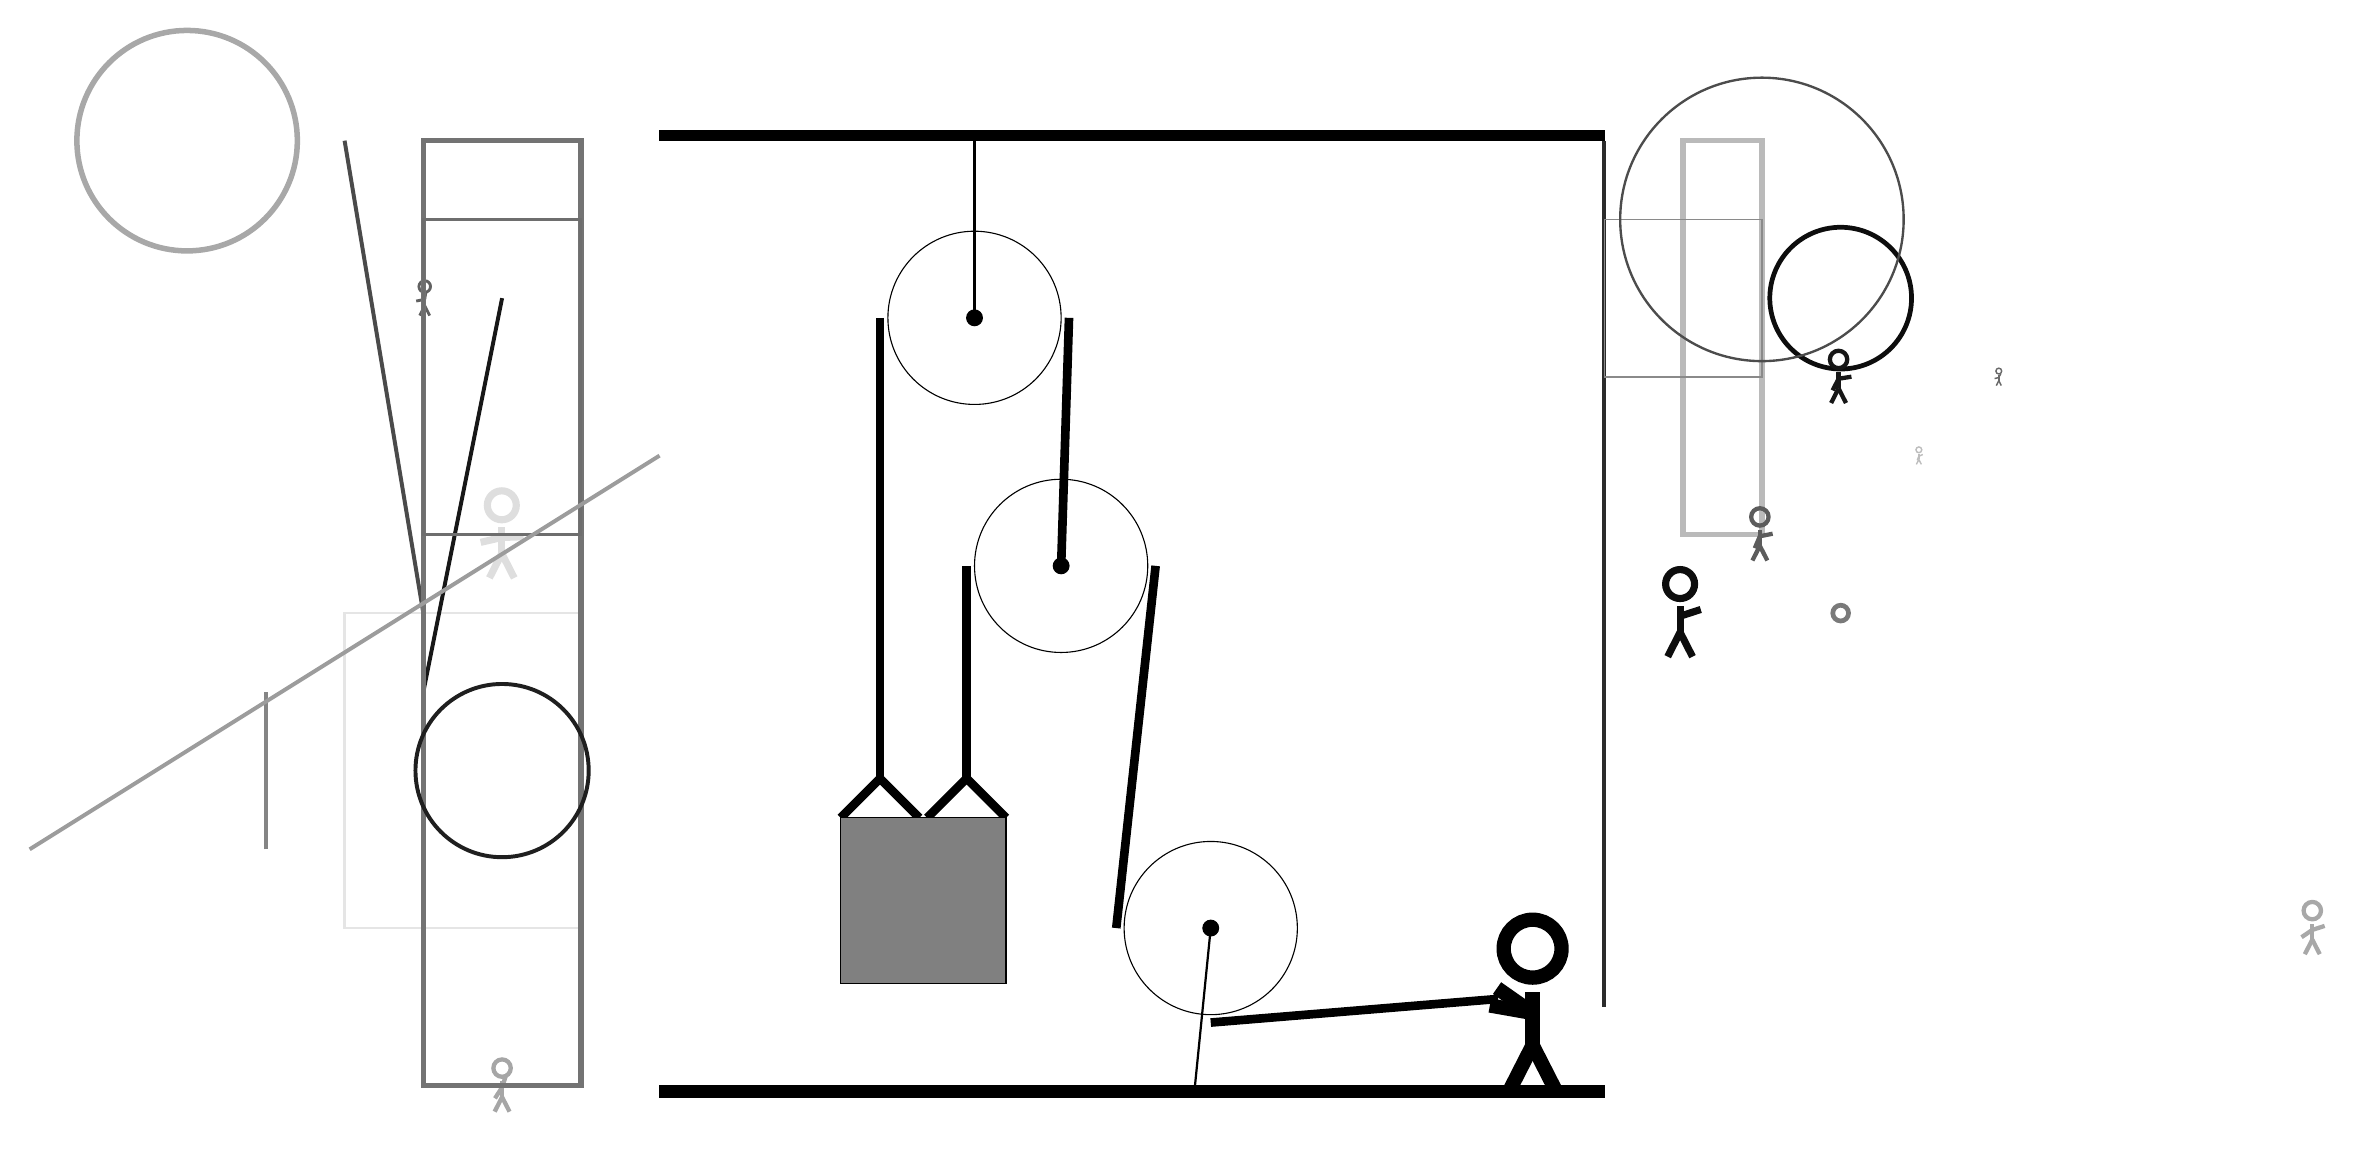
\begin{tikzpicture}
			%%%%% START %%%%%
			
			\draw[fill=black] (-2, 9) rectangle (10, 9.125);
			
			\node[line width=0.5mm, color=black!26] at (14, 5) {\Strichmaxerl[1][68][24]};
			
			\draw[line width=0.7mm, color=black!27] (12, 9) rectangle (11, 4);
			\draw[line width=0.3mm, color=black!10] (-3, -1) rectangle (-6, 3);
			\node[line width=0.6mm, color=black!62] at (-5, 7) {\Strichmaxerl[2][11][81]};
			
			\draw [line width=0.6mm, color=black!95](13, 7) circle (0.9);
			\draw[line width=0.5mm, color=black!83](10, -2) -- (10, 9);
			
			\draw[line width=0.2mm, color=black!46] (12, 8) rectangle (10, 6);
			
			\node[line width=0.2mm, color=black!91] at (13, 6) {\Strichmaxerl[3][63][9]};
			\node[line width=0.4mm, color=black!13] at (-4, 4) {\Strichmaxerl[5][13][2]};
			
			\node[line width=0.5mm, color=black!35] at (-4, -3) {\Strichmaxerl[3][57][72]};
			\draw [line width=0.3mm, color=black!70](12, 8) circle (1.8);
			\draw [line width=0.7mm, color=black!34](-8, 9) circle (1.4);
			\draw [line width=0.6mm, color=black!52](13, 3) circle (0.1);
			
			\node[line width=0.4mm, color=black!34] at (19, -1) {\Strichmaxerl[3][34][18]};
			\draw[line width=0.5mm, color=black!71](-6, 9) -- (-5, 3);
			\draw[line width=0.5mm, color=black!91](-5, 2) -- (-4, 7);
			
			\node[line width=0.4mm, color=black!59] at (15, 6) {\Strichmaxerl[1][14][63]};
			
			\draw[line width=0.7mm, color=black!55] (-3, 9) rectangle (-5, -3);
			\draw [line width=0.5mm, color=black!88](-4, 1) circle (1.1);
			\node[line width=0.3mm, color=black!95] at (11, 3) {\Strichmaxerl[5][90][18]};
			\draw[line width=0.4mm, color=black!57] (-3, 4) rectangle (-5, 8);
			
			\node[line width=0.3mm, color=black!64] at (12, 4) {\Strichmaxerl[3][67][11]};
			
			\draw[line width=0.5mm, color=black!48](-7, 0) -- (-7, 2);
			\draw[line width=0.5mm, color=black!39](-2, 5) -- (-10, 0);
			
			\draw (2, 6.75) circle (1.1);
			\draw[fill=black] (2, 6.75) circle (0.1);
			\draw[thick] (2, 6.75) -- (2, 9);
			
			\draw (3.1, 3.6) circle (1.1);
			\draw[fill=black] (3.1, 3.6) circle (0.1);
			
			\draw (5, -1) circle (1.1);
			\draw[fill=black] (5, -1) circle (0.1);
			\draw[thick] (5, -1) -- (4.8, -3);
			
			\draw[line width = 1.1mm]  (0.3, 0.4) -- (0.8, 0.9) -- (1.3, 0.4);
			\draw[line width = 1.1mm]  (1.4, 0.4) -- (1.9, 0.9) -- (2.4, 0.4);
			\draw[fill=black!50] (0.3, 0.4) rectangle (2.4, -1.7);
			
			\draw[line width = 1.1mm] (0.8, 6.75) -- (0.8, 0.9);
			\centerarc[line width = 1.1mm](2, 6.75)(0:180:1.2000000000000002);
			\draw[line width = 1.1mm] (3.2, 6.75) -- (3.1, 3.6);
			\draw[line width = 1.1mm] (1.9, 3.6) -- (1.9, 0.9);
			\centerarc[line width = 1.1mm](3.1, 3.6)(0:180:1.2000000000000002);
			\draw[line width = 1.1mm] (4.3, 3.6) -- (3.8, -1);
			\centerarc[line width = 1.1mm](5, -1)(180:270:1.2000000000000002);
			\draw[line width = 1.1mm] (5, -2.2) -- (8.65, -1.9);
			
			\node at (9, -2) {\Strichmaxerl[10][-35][170]};
			
			\draw[fill=black] (-2, -3) rectangle (10, -3.15);
			
			%%%%% END %%%%%
		\end{tikzpicture}
	\end{figure}	
\end{document}